\documentclass[a4paper,leqno,10pt]{article}
\usepackage[utf8]{inputenc}
% \usepackage{lmodern}
\usepackage{OldStandard}
\usepackage{microtype}
\usepackage[inline]{enumitem}

\usepackage{siunitx}
\usepackage{multirow}
\usepackage{subcaption}

\usepackage[english]{babel}
\usepackage[autostyle, english=british]{csquotes}
\MakeOuterQuote{"}

\usepackage{commath}
\usepackage{amsmath}
\usepackage{amsthm}
\usepackage{amssymb}
\usepackage{mathtools}

\usepackage{pgfplots}
\pgfplotsset{compat=1.11}
\usepgfplotslibrary{fillbetween}
\usetikzlibrary{patterns}
\usetikzlibrary{arrows}

\usepackage{hyperref}

\usepackage[margin=1in]{geometry}
\usepackage{changepage}
\usepackage{titlesec}
\titleformat{\section}{\normalfont\Large\bfseries\centering}{Section~\thesection:}{1em}{}

\usepackage[framemethod=tikz]{mdframed}

\def\signed #1{{\leavevmode\unskip\nobreak\hfil\penalty50\hskip2em
  \hbox{}\nobreak\hfil(#1)%
  \parfillskip=0pt \finalhyphendemerits=0 \endgraf}}
\newsavebox\mybox
\newenvironment{aquote}[1]
  {\savebox\mybox{#1}\begin{quote}}
  {\signed{\usebox\mybox}\end{quote}}

% Augmented matrices.
\makeatletter
\renewcommand*\env@matrix[1][*\c@MaxMatrixCols c]{%
  \hskip -\arraycolsep
  \let\@ifnextchar\new@ifnextchar
  \array{#1}}
\makeatother

%--------grstep
% For denoting a Gauss' reduction step.
% Use as: \grstep{\rho_1+\rho_3} or \grstep[2\rho_5 \\ 3\rho_6]{\rho_1+\rho_3}
\newcommand{\grstep}[2][\relax]{%
   \ensuremath{\mathrel{
       {\mathop{\longrightarrow}\limits^{#2\mathstrut}_{
                                     \begin{subarray}{l} #1 \end{subarray}}}}}}
\newcommand{\swap}{\leftrightarrow}

\makeatletter
\newtheoremstyle{exercise}% name of the style to be used
{5pt}% measure of space to leave above the theorem. E.g.: 3pt
{3pt}% measure of space to leave below the theorem. E.g.: 3pt
{\rm}% name of font to use in the body of the theorem
{}% measure of space to indent
{\large\bf}% name of head font
{.}% punctuation between head and body
{\newline}% space after theorem head; " " = normal interword space
{\thmname{#1}\thmnumber{ #2}\thmnote{: #3}}
\makeatother

\theoremstyle{exercise}
\newtheorem{Exercise}{Exercise}
\newenvironment{exercise}
  {\begin{mdframed}\begin{Exercise}}
  {\end{Exercise}\end{mdframed}}

\theoremstyle{plain}
\newtheorem*{thm}{Theorem}
\newtheorem*{lem}{Lemma}
\theoremstyle{definition}
\newtheorem*{defn}{Definition}
\newtheorem*{ex}{Example}
\newtheorem*{axiom}{Axiom}
\theoremstyle{remark}
\newtheorem*{rem}{Remark}

\newcommand{\df}{\textbf}
\newcommand{\T}{\mathrm{T}}
\newcommand{\F}{\mathrm{F}}
\newcommand{\IndSet}{\mathbf{I}}
\DeclareMathOperator{\cis}{cis}
\DeclareMathOperator{\arcsec}{arcsec}
\renewcommand\vec{\mathbf}

\title{Level Three Conic Sections}
\author{Alex Elzenaar}
\date{\today}

\begin{document}
\setcounter{tocdepth}{1}

\begin{titlepage}
  \maketitle
  \begin{center}
    
\includegraphics[width=0.4\textwidth]{icecream}

    \vspace{2em}

    \begin{minipage}{\dimexpr\textwidth-4cm}
      \begin{aquote}{Menaechmus}\slshape
        O King, for traveling over the country, there are royal roads and roads for common citizens, but in geometry there is one road for all.
      \end{aquote}
    \end{minipage}
  \end{center}
  \thispagestyle{empty}
\end{titlepage}
\pagenumbering{arabic}

\tableofcontents
\section*{Preface}
The conic sections are the simplest curves in the plane which are not simply straight lines. However, most secondary school treatments of the subject
tend to present a set of vaguely connected case-by-case results, rather than any kind of coherent story. These notes are my attempt to avoid this.

Most of the content is presented as a series of exercises; however, even an enthusiastic Y13 student will require a significant amount of
guidance. As always, though, it is important that the student struggles with the material on their own!

Section 2 (basic results) contains almost all the `required' material; section 3 (isometries) examines the role of transformations in geometry
in a superficial way that tries to give some idea of the fundamental concepts which tie all of the different sub-fields of geometry together.
Section 4 (cones) is a short description of the link between conic sections and cones, including an account of the `ice-cream proof' which shows
the geometric meaning of the focii of the ellipse in relation to the cone which it is a slice of. Section 5 (orthogonal families of curves) gives
a few notes on some beautiful geometry which relates different families of conics together, and section 6 (applications to physics) derives Kepler's
laws of planetary motion using L3 calculus and the theory of conics. Finally, section 7 proves a rather pretty theorem which, in some sense, tells
us everything special about the form of conic sections.

A short appendix is provided, which summarises the basic results.

\subsection*{Prerequisites}
These notes have perhaps the most `formal' prerequisites out of all my Y13 notes. I will assume results from trigonometry, linear systems, calculus, and
even algebra. However, this does not mean that the full power of these subjects are used. The most important prerequisites are actually Y11 and Y12
geometry because there are a number of results from there about triangles, circles, lines, and so forth that will be used here. My Y13 notes on trigonometry
revise a number of these results, and so the reader is directed there initially.

\begin{center}
  
\includegraphics[width=0.6\textwidth]{conics}
\end{center}

\titleformat{\section}{\clearpage\titlerule[0.8pt]\vspace{0.5ex}\normalfont\Large\bfseries\centering}{Section~\thesection:}{1em}{}[{\titlerule[0.8pt]}]
\let\oldsection\section
\renewcommand\section{\clearpage\oldsection}
\section{Introduction and Historical Remarks}
The study of the conic sections (as with much of elementary plane and solid geometry) goes back to the ancient Greeks. It is
thought that the first person to study the slices of a cone was Menaechmus, who lived on the Gallipoli Peninsula in around 350~BCE,
in his solution of the Delian problem: the construction of a cube whose volume is twice that of a given cube. Anecdotally, it is to
Menaechmus that the famous quote on the cover of these notes is attributed (usually in his disputed role as the tutor to Alexander the Great).

Euclid of Alexandria published his book \emph{Elements}, one of the most influential mathematical texts of all time, in around
300~BCE (for perspective, this is around thirty years after the death of Alexander the Great). In it, he set down the set
of basic results which can be proved true about circles and lines on a plane: while modern geometry has gone much further than
Euclid (in considering geometry in more than two dimensions, and on surfaces much more complicated than the plane), the basic
results which are taught in any introductory geometry course are usually treated in the Elements.

As well as studying circles and lines, Euclid wrote a treatise on the conic sections. Unfortunately, it no longer survives;
however, Apollonius of Perga (a city in what is now Turkey) expanded Euclid's work and published his \emph{Conics} the century
after Euclid's death. Apollonius used Euclidean geometry to prove most of the classical theorems on the conic sections, including
the many applications to physics that the subject holds.

Despite these ancient roots, it turns out that the subject is deep enough to still hold interest in the modern day. Indeed, we
will use techniques from calculus (in other words, from the 16th and 17th century) and from complex analysis (the 18th and 19th
century) in these notes; and the proper setting for conics turns out to be projective geometry, which dates from the 19th and 20th
century --- although we will only touch on this briefly here.

Conic sections have many beautiful applications; later on, we will discuss applications to optics and to celestial mechanics. For
example, in the 17th century the German astronomer Johannes Kepler showed that all astronomical bodies follow, due to gravity,
paths in the shape of conic sections.

\section{Basic results}
\begin{defn}
  Let $ O $ be a fixed point and $ \ell $ be some line not passing through $ O $. A \df{conic} $ \mathcal{C} $ is the locus of a point $ P $ such
  that, if $ K $ is the point on $ \ell $ so that $ \ell \perp PK $,
  \begin{displaymath}
    \varepsilon = \frac{\abs{OP}}{\abs{PK}}
  \end{displaymath}
  where $ \varepsilon $ is some fixed non-negative constant.

  The point $ O $ is called the \df{focus}, the line $ \ell $ the \df{directrix}, and the constant $\varepsilon$ the \df{eccentricity}.
  The \df{latus rectum} (Latin: straight side) is defined to be the chord of a conic through the focus and parallel to the
  directrix; let $ l $ be the length of the latus rectum.

  The conic is variously called:
  \begin{itemize}
    \item an \df{ellipse} if $ \varepsilon < 1 $;
    \item a \df{parabola} if $ \varepsilon = 1 $; and
    \item an \df{hyperbola} if $ \varepsilon > 1 $.
  \end{itemize}

  \begin{center}
    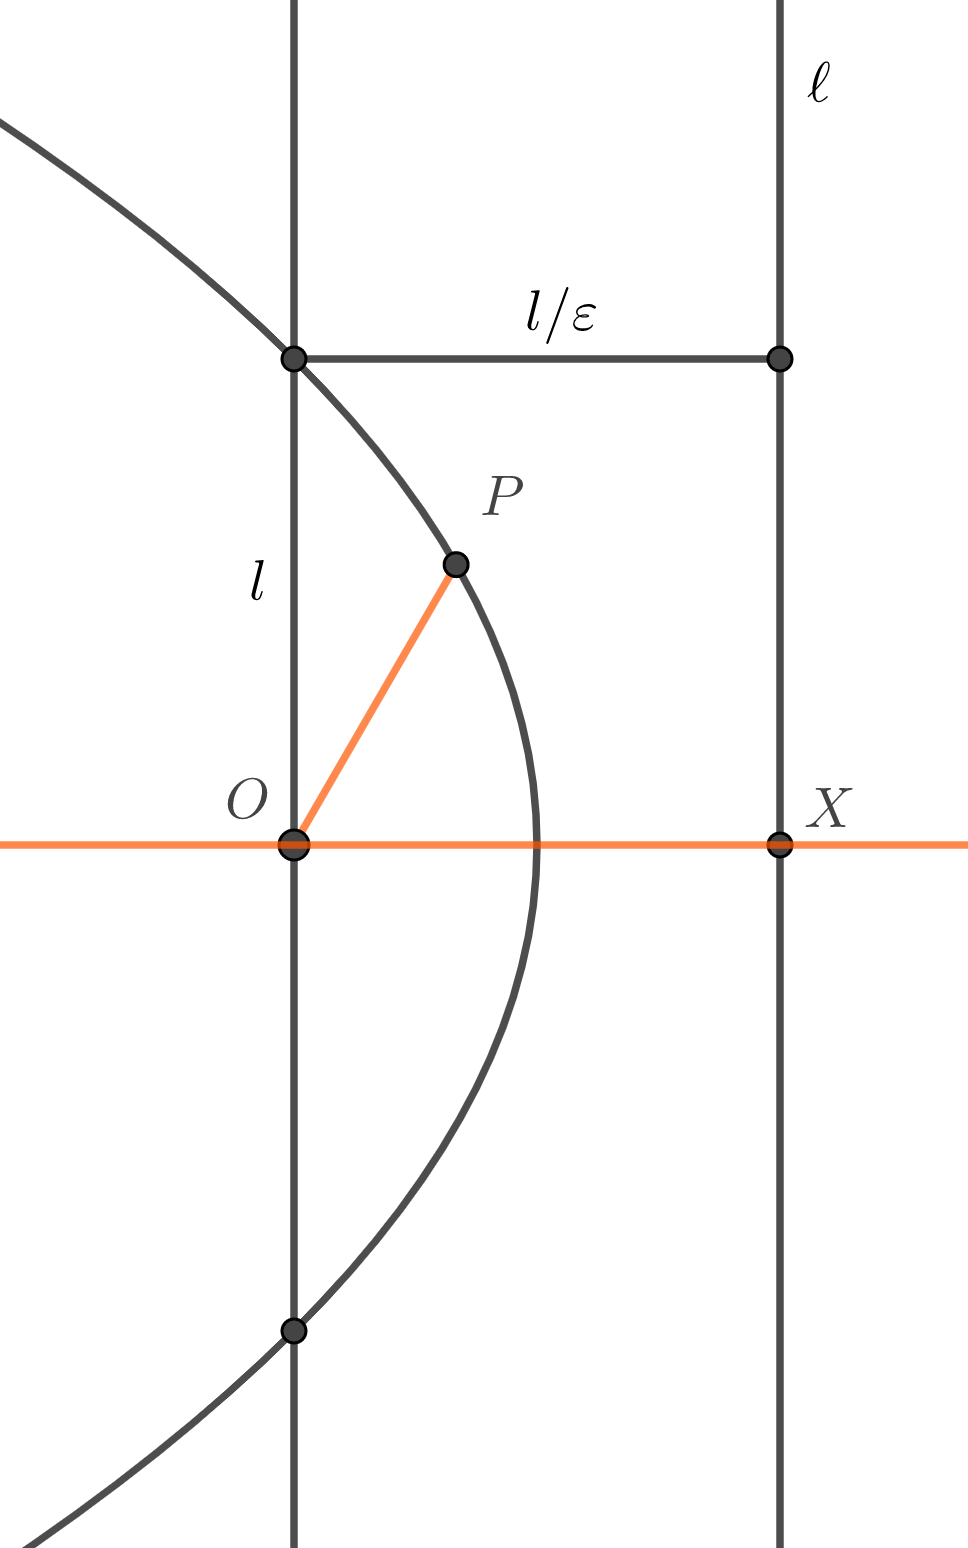
\includegraphics[width=0.3\textwidth]{polar}
  \end{center}
\end{defn}

\begin{exercise}[Polar form]
  Show that, if $ X $ is on the directrix of a conic such that $ OX \perp \ell $, then the polar equation of the
  conic with respect to this axis and origin $ O $ is
  \begin{displaymath}
    \frac{l}{r} = 1 + \varepsilon \cos \theta.
  \end{displaymath}
  Conclude that:
  \begin{enumerate}
    \item Every conic is symmetric with respect to $ OX $.
    \item The ellipse is a closed and bounded curve (i.e. it does not extend towards infinity).
    \item The parabola is unbounded, but is connected.
    \item The hyperbola consists of two seperate branches, each extending to infinity, given by $ -\alpha < \theta < \alpha $
          and $ \alpha < \theta < 2\pi - \alpha $ (where $ \alpha = \arcsec(-\varepsilon) $).
  \end{enumerate}
\end{exercise}

\begin{exercise}[Rectangular form]\label{exercise:rectangular}
  By squaring the polar form equation, show that the Cartesian equation for a conic, taking suitable axes and origin, is
  \begin{displaymath}
    x^2 + y^2 = (l - \varepsilon x)^2.
  \end{displaymath}
  \begin{enumerate}
    \item If $ \varepsilon \neq 1 $, and a suitable origin is chosen, show that the conic equation can be written in the form
          \begin{displaymath}
            \frac{x^2}{a^2} \pm \frac{y^2}{b^2} = 1
          \end{displaymath}
          for some real numbers $ a $ and $ b $. The new location of the origin is called the \df{centre} of the conic. Conclude that:
          \begin{enumerate}
            \item Both the ellipse and hyperbola are symmetric across both Cartesian axes.
            \item For an ellipse, the values $ 2a $ and $ 2b $ are the lengths of the chords through the origin along the $ x$- and $ y$-axes respectively. (The
                  longer of these is called the \df{major axis}, and the shorter the \df{minor axis}.)
            \item The two branches of a hyperbola lie in opposite regions formed by the two lines (\df{asymptotes})
                    \begin{displaymath}
                      \left(\frac{x}{a} - \frac{y}{b} \right)\left(\frac{x}{a} + \frac{y}{b} \right) = 0.
                    \end{displaymath}
                    The value $ 2a $ is the length of the transverse axis of the hyperbola and the value $ 2b $ is the length of the conjugate
                    axis: the two dimensions of the rectangle whose diagonals are the asymptotes and which is bounded by the hyperbola.
            \item Further, show that as $ x \to \pm\infty $, the branches of the hyperbola tend arbitrarily close to the asymptotes. (Hint: take limits.)
          \end{enumerate}
    \item If $ \varepsilon = 1 $, show that the conic equation for the parabola can be written in the form
          \begin{displaymath}
            y^2 = 2l(\frac{1}{2}l - x).
          \end{displaymath}
          By reflecting in a suitable vertical line, derive the standard form equation
          \begin{displaymath}
            y^2 = 2lx.
          \end{displaymath}
          Given this latter equation, give the coordinates of the focus, and the Cartesian equation of the directrix.
  \end{enumerate}
\end{exercise}

\begin{exercise}[Parametric form]
  Show that:
  \begin{enumerate}
    \item The ellipse $ x^2/a^2 + y^2/b^2 = 1 $ is parameterised by $ (a \cos t, b \sin t) $ for $ 0 \leq t < 2\pi $.
    \item The parabola $ y^2 = 2lx $ is parameterised by $ (2lt^2, 2lt) $.
    \item The hyperbola $ x^2/a^2 - y^2/b^2 = 1 $ is parameterised by $ (a \sec t, b \tan t) $ for $ 0 \leq t < 2\pi $.
  \end{enumerate}
  Illustrate these parameterisations with a suitable computer program (e.g. Geogebra, or your favourite programming language).
\end{exercise}

\begin{exercise}[Focii of rectangular conics]
  Given the equation
  \begin{displaymath}
    \frac{x^2}{a^2} \pm \frac{y^2}{b^2} = 1,
  \end{displaymath}
  compute the coordinates of the focus, equation of the directrix, and eccentricity of the conic. Hence show that
  ellipses and hyperbolae have two focii and two directrices each. Where is the directrix of a circle?

  Show that the following two properties can be used as alternative definitions for the ellipse and hyperbola:
  \begin{enumerate}[label={AP\arabic*}.]
    \item Show that the ellipse with focii $ O_1 $ and $ O_2 $ is the locus of all points $ P $
          such that $ d(O_1, P) + d(P, O_2) = R $ for some constant $ R $. Give $ R $ in terms of $ a $ and $ b $.
    \item Show that the hyperbola with focii $ O_1 $ and $ O_2 $ is the locus of all points $ P $
          such that $ d(O_1, P) - d(P, O_2) = R $ for some constant $ R $. Give $ R $ in terms of $ a $ and $ b $.
  \end{enumerate}

  As an application of this definition, we will derive the `reflection property' of the ellipse.
  \begin{enumerate}
    \item Suppose $ O_1 $ and $ O_2 $ are on the same side of a line $ \ell $. Show that the shortest path from $ O_1 $
          to $ O_2 $ which touches the line $ \ell $ is the broken line $ O_1XO_2 $, where $ X $ is on $ \ell $ and
          the angles between $ O_1 X $ and $ \ell $ and between $ X O_2 $ and $ \ell $ are equal. (Hint: you can do this
          with calculus, but that would be like killing a fly with a sledgehammer.)
    \item Show that, if $ O_1 $ and $ O_2 $ are two focii of an ellipse and $ X $ is any point on the ellipse, then the broken line $ O_1 X O_2 $
          makes equal angles with the tangent line of the ellipse at $ X $. (Hint: show that this broken line is the shortest path from $ O_1 $ to $ O_2 $
          that touches the tangent line at $ X $.)
    \item Thus, given the law of reflection for waves, show that if a light source is placed at $ O_1 $ then every ray from the source
          will arrive at $ O_2 $ at precisely the same time.
    \item Derive some result of this kind for parabolae by treating a parabola as an ellipse with one focus `at infinity'. Suggest an
          application of this property related to, say, torches.
  \end{enumerate}
\end{exercise}

\section{Isometries}
In the previous section, we saw geometrically that every ellipse or hyperbola is just a translated and rotated version of the graph of
an equation with the form
\begin{equation}
  \frac{x^2}{a^2} + \frac{y^2}{b^2} = 1.
\end{equation}
(Herein, in this section we will write $ p = 1/a^2 $ and $ q = 1/b^2 $ for convenience.)

Here, we will show this relation using coordinates --- the advantage of this approach is that it allows us to calculate precisely
from the equation of a conic its position and angle with respect to the standard axes. The subtle point here is basically that the
same curve will have different equations depending on its position in the coordinate system --- in the previous section we chose our
coordinate system in the `nicest way possible' by geometric means, and now we are given a conic already sitting in some coordinate
system which we want to understand.

In order to pursue this programme, we need to study the effect of rotations and translations on coordinate systems. We
begin with rotations because it turns out that rotating before translating is easier for our purposes.

Let $ \rho = \cis \theta $ be a complex number such that $ \abs{\rho} = 1 $. If $ z = x + yi $ is a point on the complex plane,
then $ \rho $ acts by multiplication on $ z $ to rotate it around the origin by an angle $ \theta $; we can then calculate
the resulting rectangular coordinates of $ \rho z $ to see how a rotation affects our normal coordinate system.
\begin{align*}
  z &= \abs{z} \cis(\tan^{-1} x/y)\\
  \rho z &= \abs{z} \cis(\tan^{-1} x/y + \theta)\\
         &= \abs{z} \left[\cos(\tan^{-1} x/y + \theta) + i\sin(\tan^{-1} x/y + \theta)\right].
\end{align*}

Using trig identities, we calculate
\begin{align*}
  \cos(\tan^{-1} x/y + \theta) = \cos(\tan^{-1} x/y) \cos \theta - \sin(\tan^{-1} x/y) \sin \theta\\
                               = \frac{x}{\sqrt{x^2 + y^2}} \cos \theta - \frac{y}{\sqrt{x^2 + y^2}} \sin \theta\\
  \sin(\tan^{-1} x/y + \theta) = \sin(\tan^{-1} x/y) \cos \theta + \cos(\tan^{-1} x/y) \sin \theta\\
                               = \frac{y}{\sqrt{x^2 + y^2}} \cos \theta + \frac{x}{\sqrt{x^2 + y^2}} \sin \theta
\end{align*}
and so
\begin{align*}
  \rho z &= \abs{z} \left[\cos(\tan^{-1} x/y + \theta) + i\sin(\tan^{-1} x/y + \theta)\right]\\
         &= (x \cos \theta - y \sin \theta) + i(y \cos \theta + x \sin \theta).
\end{align*}

In other words, if the point $ (x,y) $ is rotated about the origin by an angle $ \theta $, then
\begin{equation}
  (x,y) \xmapsto{\rho} (x \cos \theta - y \sin \theta,y \cos \theta + x \sin \theta).
\end{equation}

Considering $ ax^2 + bx + cxy + dy + ey^2 $, then, we want to rotate $ (x,y) $ by some $ \theta $ so that some terms vanish. Doing
a long computation, we find that
\begin{align*}
  ax^2 + bx + cxy + dx + ey^2 &\mapsto a(x \cos \theta - y \sin \theta)^2 + b(x \cos \theta - y \sin \theta)\\
                              &  \qquad + c(x \cos \theta - y \sin \theta)(y \cos \theta + x \sin \theta)\\
                              &  \qquad + d(y \cos \theta + x \sin \theta) + e(y \cos \theta + x \sin \theta)^2\\
                              &= x^2(a\cos^2 \theta + \frac{c}{2}\sin 2\theta + e\sin^2 \theta) + x(b \cos \theta + d\sin \theta)\\
                              &  \qquad + xy ((e - a)\sin 2\theta + c \cos 2\theta)\\
                              &  \qquad + y(-b \sin \theta + d \cos \theta) + y^2(a\sin^2 \theta - \frac{c}{2}\sin 2\theta + e\cos^2 \theta)
\end{align*}
and, looking at this, we see that an easy candidate we can try to get rid of is the $ xy $ term. In fact, if we want this term
to be zero we need only solve
\begin{equation}
  (e - a)\sin 2\theta + c \cos 2\theta = 0
\end{equation}
which is easy: $ \frac{-c}{e - a} = \frac{\sin 2\theta}{\cos 2\theta} = \tan 2\theta $, and so in order to remove
the $ xy $ term we need only rotate our coordinate system by
\begin{equation}
  \theta = \frac{1}{2}\tan^{-1} \frac{c}{a - e}.
\end{equation}

Making the coordinate system change $ (x,y) \mapsto (x \cos \theta - y \sin \theta,y \cos \theta + x \sin \theta) $ therefore leaves
us with something that looks like $ ax^2 + bx + dy + ey^2 = 1 $, where $ x $ and $ y $ are now coordinates in our rotated coordinate
system and where the constants $ a $ to $ e $ are not necessarily the same as before.

We already know that if $ y = f(x) $ is graphed, then we can shift the graph up by $ x_0 $ and to the right
by $ y_0 $ by suitable transformations of the coordinates: $ y - y_0 = f(x - x_0) $ has the shifted graph. Last
year, we performed similar transformations on parabolae by completing the square, and so this is the technique
which we will use now. We proceed as we did last year (but now completing the square in both $ x $ and $ y $):
\begin{displaymath}
  ax^2 + bx + dy + ey^2 = a\left(x + \frac{b}{2a}\right)^2 - \frac{b^2}{4a} + e\left(\frac{d}{2e} + y\right)^2 - \frac{d^2}{4e} = 1.
\end{displaymath}
If we now let $ (x, y) \mapsto \left(x - \frac{b}{2a}, y - \frac{d}{2e}\right) $, then we have got a coordinate
transformation that removes all the linear terms and leaves us with something like
\begin{displaymath}
  ax^2 + ey^2 = 1 + \frac{b^2}{4a} + \frac{d^2}{4e}
\end{displaymath}
and upon division of both sides by $ 1 + \frac{b^2}{4a} + \frac{d^2}{4e} $ we end up, as promised, with something of
the form $ px^2 + qy^2 = 1 $. Note that our coordinate system has completely changed: the new curve has the same
shape as our original curve, but sits inside our new coordinate system much more naturally than it sat in our old
coordinate system.

\begin{exercise}[Further thoughts on this argument]\label{exercise:degenerate}
  You are asked to think critically about the above argument (so reread it and check the computations) and to extend it (so not only must
  you read it, but understand it).
  \begin{enumerate}
    \item Clearly $ y = x^2 $ cannot be written in the canonical form. Where does the proof above fall down for a parabola?
    \item What happens if our ellipse is a circle?
    \item We have now classified the quadratic equations in two variables corresponding to hyperbolae and ellipses ($ px^2 \pm qy^2 = 1 $)
          and parabolae ($ y^2 = kx^2 $). What other forms can the graph of such a quadratic equation take? (Hint: you should be able to
          find three other kinds, and show that every quadratic equation is of one of the six kinds.)
  \end{enumerate}
\end{exercise}

\begin{exercise}[Computations]
  First, read the following quote:

  \vspace{3pt}

  \hfill\begin{minipage}{\dimexpr\textwidth-1cm}
    The attitude adopted in this book is that while we expect to get numbers out of the machine, we also expect to take action based on them, and, therefore we need to understand thoroughly what numbers may, or may not, mean. To cite the author's favorite motto,

    ``The purpose of computing is insight, not numbers,'' although some people claim,

    ``The purpose of computing numbers is not yet in sight.''

    There is an innate risk in computing because ``to compute is to sample, and one then enters the domain of statistics with all its uncertainties.''
    \begin{flushright}
      --- Richard W. Hamming, \textit{Introduction to applied numerical analysis}, McGraw-Hill 1971, p.31. (Quoted in \url{https://mathoverflow.net/a/7164}.)
    \end{flushright}
  \xdef\tpd{\the\prevdepth}
  \end{minipage}

  \begin{enumerate}
    \item Classify the following conics:
          \begin{enumerate}
            \item $ \frac{10}{4}x^2 + 3xy + \frac{10}{4}y^2 = 1 $
            \item $ 4x^2 + 24xy + 11y^2 = 5 $
          \end{enumerate}
    \item What happens to the equation for the hyperbola $ x^2 - y^2 = a^2 $ upon rotation by $ \pi/4 $?
    \item Give an equation for the parabola with vertex $ (0,2) $, and with axis $ y = x + 2 $ (opening into the positive $ x$-half plane).
    \item Find the two focii of an ellipse passing through $ (0,0) $, $ (0, 1) $, and $ (1,2) $.
  \end{enumerate}
\end{exercise}

\begin{rem}
  Felix Klein (a German mathematician who studied, among other things, geometric transformations) defined a geometry
  as a set of points together with a set of transformations of those points, such that two figures (two collections
  of points) are said to be `equivalent' if there exists some invertible transformation mapping the figures onto each other.

  For example, in normal Euclidean geometry (our current playground), we say two figures are `congruent' if they
  can be placed on top of each other to exactly cover each other: in other words (and more precisely), two figures
  are congruent if one can be mapped to the other via a series of translations, rotations, and reflections --- precisely the case
  which we have studied in this section. (Such transformations are called \emph{isometries}.) Since all these maps
  preserve lengths and angles, these things are well-defined in Euclidean geometry.

  A less familiar geometry is affine geometry, in which we also allow dilations (scaling) --- so all circles
  are equivalent in affine geometry. This does mean that lengths become meaningless: any line segment can be
  mapped onto any other line segment, no matter its length. Angles also become meaningless (why?). However, enough
  properties are left to provide a rich venue for geometry: for example, parallel lines are still parallel after an
  affine transformation, and so any result which only uses parallelism in its proof makes sense here.

  Other geometries include M\"obius geometry, where figures are equivalent if they can be mapped onto each other
  by an isometry or a circle inversion (a reflection through a circle), and projective geometry, which is a further
  loosening of the conditions on an affine geometry  such that even parallel lines make no sense and the only results
  left are those which just involve incidence and intersection. Perhaps surprisingly, projective geometry is in
  some sense the most rich geometry of all. This geometry is, in fact, the setting for section 7 of these notes.
\end{rem}

\section{Cones}
\begin{center}
  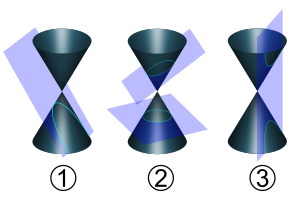
\includegraphics[width=0.5\textwidth]{slices}
\end{center}
We now move from the planar definitions of the conics to the `cone-slicing' definitions. Essentially, our goal
is to show that the conics are just slices of a cone (hence the name), as in the diagram above.\footnote{By Pbroks13 - Own work, CC BY 3.0, \url{https://commons.wikimedia.org/w/index.php?curid=5919064}}

\begin{exercise}[Defining a cone]
  We will define a cone to be the locus of all lines in three dimensional space which pass through the origin and through a point on some
  fixed curve in the plane $ z = 1 $. Note: to show a given object is a cone, one must guess a good defining curve (usually by intersecting
  it with the given plane) and then do two things: (N1) show that every line through the origin and a point on the guessed curve lies on the
  object, and (N2) show that every point on the object lies on such a line.
  \begin{enumerate}
    \item Give various non-examples of cones, especially surfaces satisfying critera N1 but not N2 and those satisfying N2 but not N1.
    \item Show that $ x^2 + y^2 = cz^2 $ is a cone whose defining curve is a circle; show that the line through the origin and the centre
          of this circle cuts the $ z = 1 $ plane at right angles. (This cone is called a \df{right circular cone}.)
    \item Show that $ ax^2 + by^2 - cz^2 = 0 $ is a cone if $ c > 0 $ and $ a $ and $ b $ are real numbers. What is its defining curve?
  \end{enumerate}
\end{exercise}

\begin{exercise}[Algebraic cone-slicing]
  Show that all six kinds of conic sections which you found in exercise \ref{exercise:degenerate} are indeed obtained by
  slicing cones with planes.

  \textit{Hints:}
  \begin{itemize}
    \item Fix a cone, say $ x^2 + y^2 = cz^2 $, and then slice it with various planes.
    \item The plane through $ (x_0, y_0, z_0) $ which is orthogonal to the line between $ (0,0,0) $ and $ (a,b,c) $ is given by
          \begin{displaymath}
            a(x-x_0) + b(y-y_0) + c(z-z_0) = 0.
          \end{displaymath}
          If you use this fact, you need not prove it.
  \end{itemize}
\end{exercise}

\begin{exercise}[Geometric cone-slicing: the icecream proof]
  In the previous exercise, we had to use coordinates to prove that every slice of a cone is a conic. We will now
  discover a geometric proof that an ellipse is just a slice of a right circular cone, in such a way that we will
  understand why such slices obey the focii properties of the ellipse.\footnote{~Tom M. Apostol, \emph{Linear Algebra: A first course} (pp.78--9). John Wiley \& Sons (1997).}

  Let us take our plane and slice our cone with it. Pick any point $ P $ in the intersection of the two surfaces (i.e.
  on the curve we wish to show is an ellipse). In addition, we will place two spheres $ S_1 $ and $ S_2 $ into our cone
  such that they are tangent to both the cone and to the plane. Let $ F_1 $ and $ F_2 $ be the two points of contact between
  the plane and the spheres, and let $ C_1 $ and $ C_2 $ be the circles of contact between the cone and the spheres.

  \begin{center}
    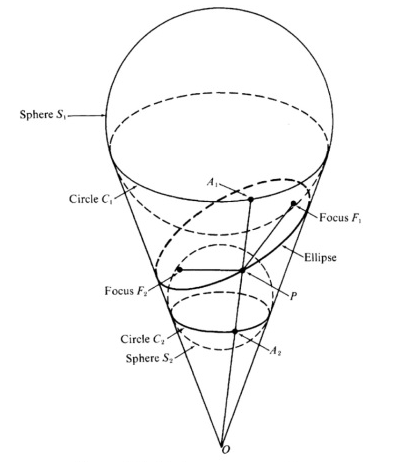
\includegraphics[width=0.5\textwidth]{apostol}
  \end{center}

  \begin{enumerate}
    \item Show that if $ X $ is a point outside some sphere, and if $ M $ and $ N $ are points on the sphere such that $ XM $
          and $ XN $ are tangent lines to the sphere, then $ \abs{XM} = \abs{XN} $. (Hint: consider the cross-section of the sphere
          obtained by slicing it with the plane of the triangle $ XMN $.)
    \item Suppose the vertex of our cone is $ O $. Show that if $ A_1 $ and $ A_2 $ are the points of intersection
          between the line $ OP $ and the two circles $ C_1 $ and $ C_2 $ then $ \abs{PF_1} = \abs{PA_1} $ and $ \abs{PF_2} = \abs{PA_2} $.
    \item Show that $ \abs{PA_1} + \abs{PA_2} $ is independent of the point $ P $.
    \item Conclude that $ \abs{PF_1} + \abs{PF_2} $ is constant for every value of $ P $, and therefore that the locus of $ P $
          is an ellipse with focii $ F_1 $ and $ F_2 $.
  \end{enumerate}
\end{exercise}

\emph{To do: same result but for hyperbolae.}

\section{Orthogonal families of conics}
In this section, we will consider families of conics with the same focii, and we will find all the curves which are orthogonal
to each family.

\begin{defn}
  Two curves are said to be \df{orthogonal} if, at every point where they intersect, they have tangent lines
  which meet at right angles. Equivalently, two curves are orthogonal if at each point of intersection the normal
  line of one is the tangent line of the other.
\end{defn}

Let us first revise a result which you should now have proved twice (both in Y12 coordinate geometry and in Y13 calculus).

\begin{exercise}[Orthogonality]
  Show that, if $ y = f(x) $ is a simple curve (i.e. a curve which does not cross itself) that is differentiable
  at $ P = (x_0, y_0) $, then there is a unique line $ N $ passing through $ P $ that is orthogonal to the curve at $ P $;
  further, the slope of $ N $ is $ -\frac{1}{f'(x_0)} $.

  If the reader is feeling clever, she should prove it in two different ways. (Hint: you can prove it via drawing
  triangles --- this is the proof given in the Y13 calculus notes --- or by rotating your line.)
\end{exercise}

\begin{rem}
  In the exercise above, we implicitly assumed in the statement that our curve was the graph of a function; however, this
  need not be the case. We only need the curve to be a function locally (i.e. for there to exist a small ball about $ (x_0, y_0) $
  within which our curve is the graph of a function). You should check that your proof only uses local properties of the graph of $ f $!
\end{rem}

\begin{exercise}[Homogenous differential equations]
  Suppose $ y $ is a function of $ x $. Recall that a differential equation is said to be \df{separable} if it can
  be written in the form $ \od{y}{x} = P(x) Q(y) $, where $ P $ and $ Q $ are functions of $ x $ and $ y $ alone.
  \begin{enumerate}
    \item Show, using the chain rule (i.e. without treating $ \od{y}{x} $ as a fraction), that $ \int \frac{1}{Q(y)} \dif{y} = \int P(x) \dif{x} $.
    \item If a curve with derivative $ \od{y}{x} = \frac{\sin x}{\cos y} $ passes through $ (0,0) $, which $ y $ values does it take when $ x = \pi $?
    \item Find an explicit formula for a function $ f $ defined for all positive numbers such that when $ y = f(x) $,
          $ \od{y}{x} = \frac{y^2}{1 - x} $ and $ f(1) = 0 $.
  \end{enumerate}

  The differential equations we wish to consider later in this section are, unfortunately, \emph{not} separable. However,
  they are nice enough that we can apply a change of variables to \emph{make} them separable.

  We say that a function of two variables $ P(x,y) $ is \df{homogenous of degree $ n $} if $ P(tx, ty) = t^nP(x,y) $ for all $ x $ and $ y $.
  \begin{enumerate}[resume]
    \item Suppose that $ P(x,y) $ and $ Q(x,y) $ are both homogenous of degree $ n $. Show that $ f(x,y) = \frac{P(x,y)}{Q(x,y)} $ is
          homogenous of degree 0.
    \item Let us consider the equation $ \od{y}{x} = f(x,y) $, where $ f $ is as in the previous question. Let $ t = 1/x $;
          show that, using the substitution $ z = y/x $ and homogeneity, we obtain the separable equation
          \begin{displaymath}
            z + x\od{z}{x} = f(1,z) = \frac{P(1,z)}{Q(1,z)}.
          \end{displaymath}
          Find the solution of this equation.
    \item Using this technique, solve $ \od{y}{x} = \frac{x^2 - 2y^2}{xy} $. (Be sure to check that the technique is applicable: i.e. that
          the right hand side is homogenous of degree zero.)
  \end{enumerate}
\end{exercise}

In a break from form, I will do a nice easy example to start with. Suppose we consider the family of curves consisting
of all the circles whose centre is the origin; it should be intuitively clear that the only curves orthogonal to all of
these circles at once are the lines through the origin.

As a first step, we know that every such circle has equation $ x^2 + y^2 = R^2 $ for some constant $ R $. Given any
particular circle, its derivative is given by $ 2x + 2y \od{y}{x} = 0 $ or $ \od{y}{x} = -\frac{x}{y} $; since the
parameter $ R $ is absent from this equation, it describes every such circle. (We have shown that every such circle
has this derivative, but you should check yourself, by integrating, that every equation of this form is a circle centred
at the origin.)

We want to find all the curves such that, at every point $ (x,y) $ on our curve, the tangent line of our curve is the
normal line of the circle centred at the origin and passing through that point. To do this, we simply need to solve
\begin{displaymath}
  \od{y}{x} = \frac{y}{x}
\end{displaymath}
and this is not only separable but easy: $ \int \frac{\dif{y}}{y} = \int \frac{\dif{x}}{x} $ and thus $ \ln\abs{x} = \ln\abs{y} + C $,
or $ x = Ky $; and this is just the family of all lines through the origin, as we guessed initially.

For convenience, if $ \mathcal{F} $ is a family of curves then we will call the family of curves orthogonal to $ \mathcal{F} $
the \df{orthogonal complement} of $ \mathcal{F} $.

\begin{exercise}[Orthogonal families of curves]
  We (or rather you, the reader) will now show that when we take orthogonal complements of various families of conics, then we obtain
  other families of conics. As well as the results explicitly stated here, you should consider how the families are related to each
  other. Show that:
  \begin{enumerate}
    \item The family of NE-SW diagonal hyperbolae, $ xy = c $, are orthogonal to the family of NW-SE diagonal hyperbolae, $ xy = -c $.
    \item The vertical parabolae, $ y = ax^2 $, are orthogonal to the family of ellipses $ x^2 + \frac{y^2}{b} = 1 $. (See \texttt{parabolae-and-ellipse.ggb}.)
    \item The family of all circles tangent to the $ y$-axis at the origin (i.e. $ x^2 + y^2 = 2rx $) is orthogonal to the family of all circles tangent to
          the $ x$-axis at the origin (i.e. $ x^2 + y^2 = 2ry $).
  \end{enumerate}
  Hence, complete the following: orthogonal complements of $ X $ are $ Y $, taking $ X $ to be hyperbolae, parabolae, circles, and ellipses. (We have
  found the orthogonal complements of families of curves in particular places, but consider the hint after exercise \ref{ex:apollonius}.)
\end{exercise}

Finally, we have one rather pretty example.
\begin{exercise}[Circles of Apollonius]\label{ex:apollonius}
  Fix two points $ A $ and $ B $. Let us consider the locus of all points $ P $ such that $ \frac{\abs{AP}}{\abs{BP}} = \rho $, for positive numbers $ \rho $;
  we will examine one particular perpendicular family.
  \begin{enumerate}
    \item Show that if we fix $ A $ and $ B $ and vary $ \rho $ then we have a family of circles whose centres lie on the line $ AB $.
    \item Show that the orthogonal complement of this family is the set of circles passing through $ A $ and $ B $ with centres on the perpendicular
          bisector of the segment $ AB $.
    \item Use Geogebra (or similar software) to draw a nice picture.
  \end{enumerate}

  Hint: without loss of generality, you can suppose $ A = (-1, 0) $ and $ B = (0, 1) $. (Then the result follows for any choice of $ A $ and $ B $,
  simply because dilations, translations, and rotations all preserve circles and orthogonality of lines.)

  There are three ways to do this exercise that the author is aware of: perhaps the easiest for us now is to apply calculus like we have been
  doing throughout this section. For a geometric view on this exercise, see Coxeter \S 6.6; for a view from complex calculus, see Fisher \S 1.2.
\end{exercise}

\begin{exercise}[Bipolar coordinates (difficult)]
  (Prerequisite: you do need to understand exercise \ref{ex:apollonius} quite well. You should also read the epilogue on hyperbolic trigonometric
  functions in the trigonometry notes.)

  From your pictures in the previous exercise, you should notice that every point in the plane is at the intersection of two circles of Apollonius.
  Let us fix $ A = (-1, 0) $ and $ B = (1,0) $, as in the hint for the previous exercise; we will use these circles to define a new coordinate system
  for the plane.

  Suppose $ P = (x,y) $ lies at the intersection of two circles; then we define $ \sigma $ to be the angle $ APB $, and $ \tau = \ln \frac{\abs{PA}}{\abs{PB}} $.
  We then define the \df{bipolar coordinates} of $ P $ to be $ (\sigma, \tau) $.
  \begin{enumerate}
    \item Show that
          \begin{displaymath}
            \begin{cases}
              x = \frac{\sinh \tau}{\cosh \tau - \cos \sigma}\\
              y = \frac{\sin \sigma}{\cosh \tau - \cos \sigma}.
            \end{cases}
          \end{displaymath}
    \item Identifying the plane $ \mathbb{R}^2 $ with the complex numbers $ \mathbb{C} $, show that this is
          equivalent to $ x + iy = ai \cot \left(\frac{\sigma + i\tau}{2}\right) $. (Recall that we define $ \cot z = \frac{e^{iz} - e^{-iz}}{ie^{iu} + ie^{-iu}} $.)
    \item Identify the locus of all $ P = (\sigma, \tau) $ such that (a) $ \sigma $ is held constant, or (b) $ \tau $ is held constant.
    \item Translate the standard equations of the conics into bipolar coordinates.
  \end{enumerate}
\end{exercise}

\section{Applications to physics}
We will now look briefly at some applications to the theory of gravity. Recall from stage 2 physics (or earlier)
the following definitions and results:

\begin{defn}\leavevmode
  \begin{enumerate}
    \item If an object's position $ x $ is given as a function of time $ t $, then $ v := \od{x}{t} $ is known as
          the velocity of the object and $ a := \od{v}{t} = \od[2]{x}{t} $ is known as the acceleration of the object.
    \item Newton's second law of motion: An object with mass $ m $, when acted upon by a force $ F $, undergoes an acceleration $ a = F/m $ in
          the same direction as the force; the force does not affect the motion of the object in any other direction.
    \item Newton's law of gravity: If two objects have masses $ M $ and $ m $ and their centres are a distance $ R $ apart, then they impose
          on each other equal and opposite forces of magnitude $ \frac{GMm}{R^2} $, where $ G $ is a constant.
    \item If an object of mass $ m $ is close to the surface of the earth, then the gravitational force upon it
          due to the earth is $ mg $ towards the centre of the planet, where $ g \approx 9.81 $.
  \end{enumerate}
\end{defn}

As a warmup, we will derive some simple results from stage 2 physics.

\begin{exercise}[Projectile motion]
  An object of small mass $ m $ flying through the air can often be modelled as a \df{projectile}: a particle
  with constant speed $ v_x = \od{x}{t} $ along the ground, and constant acceleration $ a_y = mg $ pointing
  towards the centre of the earth.

  \begin{enumerate}
    \item Show that the motion of the mass is a parabola.
    \item If the object is launched skywards at an angle of $ \pi/4 $ to the horizontal, with a
           velocity $ v = 10 $ along its direction of travel, how far along the ground will it travel?
    \item With the conditions of problem (2), how is the focus of the parabola traced positioned?
    \item At what angle must the object be launched for the focus to lie precisely on the ground?
  \end{enumerate}
\end{exercise}

So, to a first approximation, objects follow a parabolic path due to gravity. We made two main simplifications here:
\begin{enumerate}
  \item We assumed that the force of gravity on the object was constant (in both magnitude and direction) regardless of position.
  \item We assumed that the earth was fixed in space relative to the object.
\end{enumerate}

Because of the positioning of our object, these approximations are actually quite valid: the force of gravity
is roughly perpendicular to the surface of the earth, the surface of the earth is approximately flat when you are close
to it, and the object was far enough away from the centre of the earth for a small increase or decrease in height
to have a negligible impact on the magnitude force felt by the object. Further, the earth is massive compared to our
object and so would feel a negligible force due to it.

We will now relax the first of these two approximations, and consider the new path followed.\footnote{For a detailed
exposition of this derivation, see Simmons \S21.}
\begin{exercise}[Kepler's laws]
  In order to make our discussion more concrete, we will fix some large mass $ M $ at the origin $ O $, and we
  will consider some smaller planet, located at $ \vec{r} $ with mass $ m $. The planet $ P $ will accelerate due to
  the gravitational force exerted on it by $ O $; we want to study the motion of $ P $. It is convenient to use
  polar coordinates.

  \begin{enumerate}
    \item Kepler's second law.
      \begin{enumerate}
        \item Suppose that $ \vec{u}_r = (\cos \theta, \sin \theta) $ is the unit vector in the direction of $ \vec{r} $, so $ \vec{r} = r\vec{u}_r $.
              Let us define $ \vec{u}_\theta = (-\sin\theta, \cos \theta) $ to be the unit vector perpendicular to $ \vec{u}_r $ in the direction
              of increasing $ \theta $. Show that $ \od{\vec{u}_r}{\theta} = \vec{u}_\theta $ and $ \od{\vec{u}_\theta}{\theta} = -\vec{u}_r $, and hence (using
              the product and chain rules) deduce that:
              \begin{gather*}
                \vec{v} = \od{\vec{r}}{t} = r \od{\theta}{t} \vec{u}_\theta + \od{r}{t} \vec{u}_r\\
                \vec{a} = \od{\vec{v}}{t} = \left( \od[2]{r}{t} - r \left(\od{\theta}{t}\right)^2 \right)\vec{u}_\theta.
              \end{gather*}
        \item Hence, using Newton's second law of motion and (a) above, we can write expressions for the components of the
              force $ \vec{F} = F_\theta \vec{u}_\theta + F_r \vec{u}_r $ acting on an object of mass $ m $:
              \begin{gather*}
                F_\theta = m\left(r \od{\theta}{t} \vec{u}_\theta + \od{r}{t} \right)\\
                F_r = m\left( \od[2]{r}{t} - r \left(\od{\theta}{t}\right)^2 \right).
              \end{gather*}

              Our force of gravity is a \df{central force}: it only acts in the direction of $ \vec{r} $. Hence the $ \theta$-component
              of the force acting on the mass $ m $ is zero. Show that
              \begin{displaymath}
                r^2 \od{\theta}{t} = h
              \end{displaymath}
              for some constant $ h $.
        \item Suppose $ A(t) $ gives the area `swept out' by the radius vector $ \vec{r} $ between some fixed time $ t_0 $
              and the time $ t $. Using the fact that $ \od{A}{\theta} = \frac{r^2}{2} $ (since $ \dif{A} = \pi r^2 \cdot \frac{\dif{\theta}}{2\pi} $),
              show that $ A(t_2) - A(t_1) = \frac{1}{2}h(t_2 - t_1) $. Conclude \df{Kepler's second law}: if $ P $ and $ Q $ are
              planets with associated masses $ m_P $ and $ m_Q $, then over a time $ \Delta t $ the planets will sweep out equal
              area.
      \end{enumerate}
    \item Kepler's first law.
      \begin{enumerate}
        \item Let $ z = 1/r $. Express $ \od{r}{t} $ and $ \od[2]{r}{t} $ in terms of $ \od{z}{\theta} $ and $ \od[2]{z}{\theta} $.
        \item By Newton's law of gravity, $ F_r = -\frac{GMm}{r^2} $. Thus, we have that $ \od[2]{r}{t} - r \left(\od{\theta}{t}\right)^2 = -\frac{GM}{r^2} $.
              Use the expression in (1b) above to show that $ \od[2]{r}{t} - \frac{h^2}{r^3} = -\frac{GM}{r^2} $, and then apply
              the substitution in (a) to show that $ \od[2]{z}{\theta} + z = \frac{GM}{h^2} $.
        \item Solve the differential equation in (b). (Hint: the general solution is $ z = A \sin \theta + B \cos \theta + \frac{GM}{h^2} $.)
        \item Let us shift and rotate our coordinate axis such that $ \vec{r} $ is minimised when $ \theta = 0 $: in other words, we pick
              our axis such that the mass $ m $ is closest to the origin at $ \theta = 0 $. Since $ 1/r $ is maximised when $ r $ is minimised,
              we have that $ \eval{\od{z}{\theta}}_{\theta = 0} = 0 $ and $ \eval{\od[2]{z}{\theta}}_{\theta = 0} < 0 $. Show that $ A = 0 $
              and $ B > 0 $.
        \item Further, show that
              \begin{displaymath}
                r = \frac{h^2/GM}{1 + (Bh^2/GM)\cos\theta};
              \end{displaymath}
        \item Write $ e = Bh^2/GM $ in the equation of (e), and conclude \df{Kepler's first law} by comparison
              with exercise 1: the locus of $ P $ is a conic section with one focus $ O $.\footnote{It can be shown
              that $ e = \sqrt{1 + E \frac{2h^2}{G^2M^2m}} $, where $ E $ is the potential energy associated with the mass $ m $; so
              the particular conic traced depends on the energy associated with the mass $ m $. Thus the planets in
              the solar system, which have negative energy (they are trapped by the sun, and work must be done to them
              to pull them away), trace elliptical orbits; while bodies like comets trace parabolic and hyperbolic trajectories.}
      \end{enumerate}
    \item Kepler's third law.
      \begin{enumerate}
        \item Suppose our mass traces an elliptical orbit, such that $ Bh^2/GM < 1 $ in the equation $ r = \frac{h^2/GM}{1 + (Bh^2/GM)\cos\theta} $.
              Let us write this in rectangular form as $ \frac{x^2}{a^2} + \frac{y^2}{b^2} = 1 $. Using results from exercises 1 and 2 (collected
              in the appendix), show that $ a = \frac{h^2a^2}{GMb^2} $ and thus that $ b^2 = \frac{h^2a}{GM} $. (Hint: $ a $, the semi-major axis
              length, is half the sum of the maximum and minimum values for $ r $.)
        \item If $ T $ is the period of revolution of our mass $ m $, use Kepler's second law (in particular the formula derived in (1c)) to show
              that $ \pi ab = \frac{hT}{2} $ and thus, using (a), that $ T^2 = \left(\frac{4\pi^2}{GM}\right)a^3 $. Noting that this is independent
              of the mass $ m $, conclude \df{Kepler's third law}: the square of the period of revolution of any planet is proportional
              to the cube of its average distance from the sun, where the constant of proportionality depends only on the mass $ M $ and
              some constants of nature.
      \end{enumerate}
  \end{enumerate}
\end{exercise}

\section{The intersection theorem}
\begin{center}
  \emph{You know, for a mathematician, he did not have enough imagination. But he has become a poet and now he is fine.} --- Hilbert (on an ex-student)
\end{center}
We will study in this topic precisely equations of the form
\begin{equation}\label{eqn:prototype}
  ax^2 + 2hxy + by^2 + 2gx + 2fy + c = 0;
\end{equation}
This class of equations is the class of \df{quadratic equations} (in two variables). Note that, without loss
of generality, we can assume $ c = 1 $ (otherwise, we just divide through by $ c $).

The set of all points $ (x,y) $ satisfying a quadratic equation is called a \df{curve of the second degree}; we
have already implicitly shown that every conic is a curve of the second degree, and in exercise \ref{exercise:degenerate}
you classified all the other types of such curve.

Our main theorem is a generalisation of the statement from algebra that every quadratic equation in one variable
(i.e. every equation $ x^2 + px + q = 0 $) has precisely two solutions (if you count correctly).
\begin{thm}\label{thm:funthmquad}
  Every line meets a curve of the second degree in precisely two points.
\end{thm}

This theorem is very nice, but (like the proof for quadratics in one variable) we do have to make a trade:
we have to take our coordinate system to be over the complex numbers. Thus, for the remainder of this section,
we will assume implicitly that rather than living in the real plane $ \mathbb{R}^2 $ we are in fact living
in the complex plane $ \mathbb{C}^2 $. In some sense, then, we are doing geometry in four dimensions. On the
other hand, in many places we will only be interested in real coordinates. For example, the graph of a four-dimensional
object is a little tricky to draw if we only have three dimensions available!

The proof of the theorem will take a few pages; the theorem is quite `deep',\footnote{The mathematical meaning of `deep' is hard to pin down: it sometimes
means ``I know this proof and you don't'', or perhaps ``I don't really understand this proof'', or even ``some celebrity/lecturer/textbook author once
told me it was deep''. In this case, I am using it to mean that the proof is difficult and is something of a gateway into an entirely new type of geometry.}
and so it is absolutely normal to expect the going to be slow.

Our first proof attempt looks all right, and indeed it is almost correct;

\begin{proof}[Proof attempt]
  Let $ ax + by = 1 $ be our line. At least one of $ a $ or $ b $ is non-zero; assume that $ a $ is
  non-zero (but essentially the same proof will work if $ a = 0 $ but $ b $ is non-zero). Then we
  can substitute $ x = \frac{1 - by}{a} $ into our curve of the second degree to obtain a quadratic
  equation in the variable $ y $; by the fundamental theorem of algebra, this equation has two solutions;
  and each of these corresponds with a point of intersection.
\end{proof}

The problem with this proof is illustrated by the following example:-
\begin{ex}
  Consider the quadratic $ xy + y + x^2 = 1 $. This describes a perfectly good curve in two dimensions, graphed here.
  \begin{center}
    \fbox{\begin{tikzpicture}
      \begin{axis}[
        axis lines = center,
        xlabel = $ x $,
        ylabel = $ y $
      ]
        \addplot[domain = -5:5, color = red] {1-x};
        \draw[color = red] ({axis cs:-1,0}|-{rel axis cs:0,0}) -- ({axis cs:-1,0}|-{rel axis cs:0,1});
      \end{axis}
    \end{tikzpicture}}
  \end{center}
  If we intersect this curve with the line $ y = 2 - x $, then we obtain a linear equation $ x + 2 = 0 $ instead of a quadratic
  equation --- and so even counting multiplicities and moving up to $ \mathbb{C} $, we only have one solution.
\end{ex}

The reader might be tempted to discount this example as uninteresting, because it's simply the intersection of a pair of two lines
with a third line and thus isn't really a problem that affects our programme of studying conics.

The next example, though, is both more fundamental and more worrying.
\begin{ex}
  If we intersect the parabola $ x^2 = y $ with the line $ x = 0 $, we obtain a single point of intersection, even
  up to multiplicity.
\end{ex}

Does this mean that we have to abandon the beautiful intersection theorem?

It turns out that, like how we expanded our number system to make the fundamental theorem of algebra work
nicely, we can expand our plane $ \mathbb{C}^2 $ further to make our intersection theorem work.

We will not make this precise, but the method we will use is some kind of limiting process; the result, and the
system we will work in from now on, is the projective plane over $ \mathbb{C} $. Let us see how we climb to it.

\subsection{Euclidean geometry}
It turns out that in order to approach some kind of resolution, we need to mention the elephant in the room: the
foundation of all the geometry which we have been doing thus far in our mathematical lives. (This might seem at first
glance completely unrelated to the algebraic problem we're trying to solve, but bear with me.)

As I mentioned in the historical introduction, Euclid of Alexandria set down in around 300~BCE a set of basic results
which can be proved true about circles and lines on a plane in his treatise \textit{Elements}.
Euclid was influential because he was the first author (or, more likely, the first author whose work survives) to
attempt to rigorously prove all his results based on a set of `universal truths': a set of simple statements (called
\df{axioms}) whose truth is self-evident. In some sense, the goal of mathematics is to deduce the behaviour of the
most complicated systems possible from the simplest axioms possible.\footnote{The axiom system which most of modern
mathematics is done within is called ZFC (Zermelo-Fraenkel with Choice, named after two mathematicians working on the
area in the early 1900s).} Euclid's axioms were as follows:
\begin{enumerate}
  \item A straight line segment can be drawn joining any two points.
  \item Any straight line segment can be extended indefinitely in a straight line.
  \item Given any straight line segment, a circle can be drawn having the segment as radius and one endpoint as center.
  \item All right angles are congruent.
  \item Given any straight line and a point not on it, there exists one and only one straight line which passes through
        that point and never intersects the first line, no matter how far they are extended.
\end{enumerate}
Putting aside the fact that these axioms are in fact insufficient for the purpose of constructing plane geometry, it is
clear that the fifth axiom is both far less elegant than the others and far more complicated. Indeed, Euclid himself avoided
using it in his proofs except where necessary (he avoids it completely for the first 28 propositions, for example) and for
many years mathematicians believed that it was in fact a theorem: that it could be proved from the previous four axioms.

It turns out that this is false: there exist geometries for which the fifth axiom is false (for example, on a sphere).

\subsection{Projective geometry}
The mathematical world which we are interested in is known as \df{projective geometry}; the name relates to the original
applications, which were related to perspective in drawings. We obtain this geometry by replacing Euclid's final axiom with the following axiom:
\begin{axiom}[Elliptic incidence property]
  Any two distinct lines in a projective geometry meet at exactly one point.
\end{axiom}
This is clearly not true in usual Euclidean geometry. On the other hand, we didn't let this kind of thing stop us in the
past: the number $ i $ is absolutely useless for counting sheep, for example, but that doesn't stop the complex numbers from
being an interesting (and useful) mathematical space.

The complex numbers became much clearer once we stopped thinking about numbers as a line and started drawing them as a plane. There
is an analogous simple way to construct and think about a projective plane by extending the Euclidean plane (and then extending our
setting, the complex plane, will be done in the same way).

When we think about it, we find that the only reason that Euclidean geometry doesn't satisfy this axiom is that parallel lines exist.
We will therefore \emph{define them not to exist}!

More precisely, given every set of parallel lines with slope $ m $, we will take our plane and add on a new point $ \infty_m $ called
a \emph{point at infinity}, and then define this new point to be on all the lines with slope $ m $. Thus, these parallel lines now
intersect at exactly one point (the point at infinity related to their slope) and all other lines intersect in exactly one point (the
same place they did before).

\begin{center}
  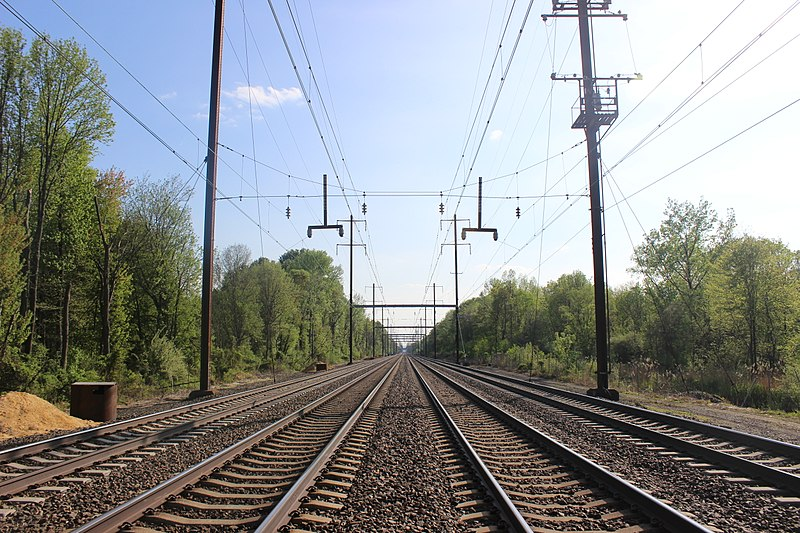
\includegraphics[width=0.5\textwidth]{vanishingpoint}
\end{center}

This can be made to make some sense physically, and indeed the first place which projective geometry appeared was when Renaissance artists
like Leonardo da Vinci began to experiment with perspective drawing --- if you look down two parallel lines in real life, like those in the
image above,\footnote{© Vespertunes / Wikimedia Commons / ``Vanishing Point of Railway''. \url{https://commons.wikimedia.org/wiki/File:Vanishing_Point_of_Railway.jpg}}
they appear to meet at the horizon, and lines going in the same direction away from you (i.e. lines with the same slope) meet
at the same point. We call the line joining all the points at infinity (in this physical case, the horizon) the \df{line at infinity}.

Going back to our problem of curves of the second degree, let us consider our second example: $ x^2 = y $ only intersects the line $ x = 0 $
at one point.

\begin{center}
  \fbox{\begin{tikzpicture}
    \begin{axis}[
      axis lines = center,
      xlabel = $ x $,
      ylabel = $ y $, ymin=-2
    ]
      \addplot[domain = -5:5, color = red] {x^2};
      \draw[color = blue] ({axis cs:0,0}|-{rel axis cs:0,0}) -- ({axis cs:0,0}|-{rel axis cs:0,1});
    \end{axis}
  \end{tikzpicture}}
\end{center}

But notice, as $ x \to \pm \infty $ the curve $ x^2 $ tends towards being vertical! More precisely, we have
that $ \lim_{x \to \infty} \od{}{x} x^2 = \infty $; thus, the parabola is \df{eventually parallel} to the
vertical line, and so the two intersect for a second time at the point at infinity $ \infty_\infty $.

This is even more blatant in our first example: we had the following curve (and again, the blue line is the
line we intersect with our second degree curve):

\begin{center}
  \fbox{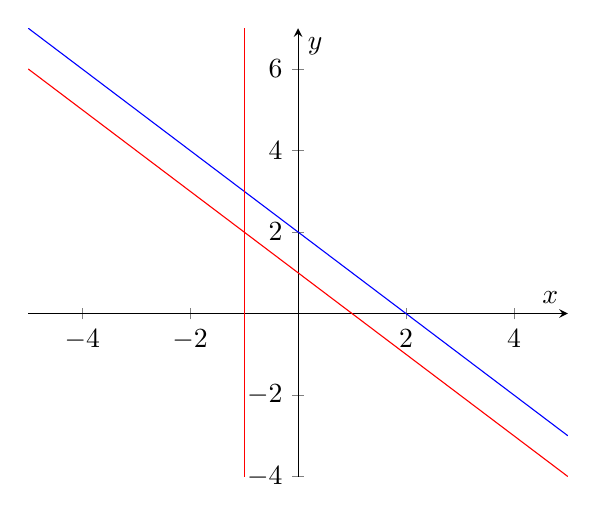
\begin{tikzpicture}
    \begin{axis}[
      axis lines = center,
      xlabel = $ x $,
      ylabel = $ y $
    ]
      \addplot[domain = -5:5, color = red] {1-x};
      \addplot[domain = -5:5, color = blue] {2-x};
      \draw[color = red] ({axis cs:-1,0}|-{rel axis cs:0,0}) -- ({axis cs:-1,0}|-{rel axis cs:0,1});
    \end{axis}
  \end{tikzpicture}}
\end{center}

In this case, the curve is not only \emph{eventually} parallel, but in fact it is \emph{actually} parallel!

The picture to keep in mind, for curves of the second degree at least, is the following.

\begin{center}
  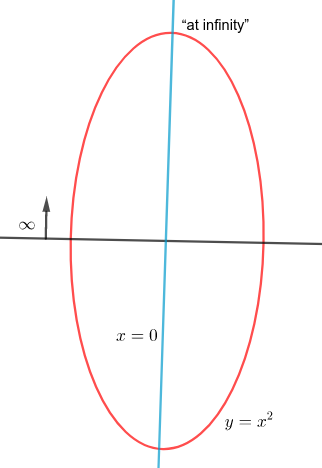
\includegraphics[width=0.3\textwidth]{infiniteparabola}
\end{center}

Note that this picture does not actually reflect what is \emph{really} going on when we graph second degree
equations in the plane --- it's a diagrammatic representation of the fact that we've made a fundamental extension
to our system of geometry (and to our system of algebra, but this isn't visible on a real graph).

Philosophically, all we've done is decided what property we want our algebro-geometric system to have (that
curves of the second degree intersect any line at exactly two places, unless it's tangent to the line) and then
invented a geometry in which this property is true. It turns out that this geometry has a lot of other beautiful
properties, most of which we don't have time to look at --- but at this stage, it's completely synthetic. We simply
arbitrarily added a bunch of points (and we're honestly lucky we didn't get any contradictions). In fact, eventually
we will see that there is an incredibly natural way to construct a projective plane without having to worry about
sticking in a bunch more points and cooking it ourselves.

For now, we will content ourselves with proving our motivational theorem.

\subsection{Proof of the main theorem}

Let $ y = mx + n $ be our line. Then we can substitute $ y $ into our curve of the second degree to obtain an equation
in the variable $ x $ which is either of degree 1 or degree 2. (If necessary, let $ m $ be infinite.)

\paragraph{Case I.} If the equation is of degree two, then by the fundamental theorem of algebra it
has two solutions; and each of these corresponds with a point of intersection. (If the line is tangent
to our curve, then we still get two solutions but they happen to be the same; in some sense, this is
just because the tangent line does intersect twice, but at the same point.)

\paragraph{Case II.} We will be done if we can show the following: if a line $ y = mx + n $ intersects
some quadratic equation $ ax^2 + 2hxy + by^2 + 2gx + 2fy + c = 0 $ in exactly one point (i.e. in such a
way as to produce a linear equation in $ x $ rather than a quadratic) then
\begin{equation}
  \lim_{x \to \infty} y'(x) = m.
\end{equation}
(where the derivative is of the quadratic equation), because in this case both the conic
and the line can be said to intersect at the `point at infinity' $ \infty_m $.

\begin{lem}
  This limit always exists whenever $ x $ can be made to go to infinity.
\end{lem}
\begin{proof}
  This was actually proved in exercise \ref{exercise:rectangular}: in the case of a hyperbola, it tends
  to its asymptotes. The only other unbounded conics are the degenerate ones from \ref{exercise:degenerate};
  the unbounded curves here are just unions of lines, and so have constant derivatives at each point.
\end{proof}

We will begin by finding the condition on the coefficients of our quadratic for $ x^2 $ to vanish upon substitution.
So let us substitute $ y = mx + c $ into our quadratic; we obtain
\begin{displaymath}
  ax^2 + 2hx(mx + c) + b(mx + c)^2 + 2gx + 2f(mx + c) + c = 0.
\end{displaymath}

Expanding, and setting the coefficient of the $ x^2 $ term to zero, we find that
\begin{displaymath}
  a + 2mh + bm^2 = 0.
\end{displaymath}

We will find the derivative $ y'(x) $; this is a simple exercise in implicit differentiation and we get that
\begin{displaymath}
  \od{y}{x} = -\frac{ax + hy + g}{hx + by + f}.
\end{displaymath}
Substituting our condition on the coefficients, we have
\begin{displaymath}
  \od{y}{x} = -\frac{-2mhx - bm^2x + hy + g}{hx + by + f}.
\end{displaymath}

Step 3. Taking limits of both sides, we have
\begin{displaymath}
  \lim_{x \to \infty} \od{y}{x} = \lim_{x \to \infty} -\frac{-2mhx - bm^2x + hy + g}{hx + by + f}.
\end{displaymath}

It is not immediately obvious how we should deal with this right-hand side, because $ y $ also depends
on $ x $. Looking at the equation for the quadratic, we note that as $ x \to \infty $, we must have $ y \to \pm\infty $ ---
otherwise the right hand side couldn't stay at zero. Therefore, both the top and the bottom of the fraction under our
limit go to infinity; we can apply the following theorem about limits:

\begin{thm}[l'Hopital's Rule]
  If $ \lim_{x \to \infty} f(x) = \infty $ and $ \lim_{x \to \infty} g(x) = \infty $, and if $ \lim_{x\to\infty} f'(x)/g'(x) = l $,
  then $ \lim_{x\to\infty} f(x)/g(x) = l $.
\end{thm}
\begin{proof}
  Omitted. See any book on single-variable calculus, for example Spivak, chapter 11, theorem 9 and exercises 36--38.
\end{proof}

Let $ \lim_{x \to \infty} \od{y}{x} = L $. Then we have
\begin{displaymath}
  L = \lim_{x \to \infty} -\frac{-2mhx - bm^2x + hy + g}{hx + by + f} = \lim_{x \to \infty} -\frac{-2mh - bm^2 + h\od{y}{x}}{h + b\od{y}{x}}
                                                                      = -\frac{-2mh - bm^2 + hL}{h + bL}
\end{displaymath}
and $ 0 = bL^2 + 2hL - 2mh - bm^2 $, so
\begin{displaymath}
  L = \frac{-2h + \sqrt{4h^2 + 4b(2mh + bm^2)}}{2b} = \frac{-2h + 2\sqrt{h^2 + 2bmh + bm^2}}{2b}
                                                    = \frac{-2h + 2(h + bm)}{2b} = m
\end{displaymath}
Thus we have shown that if the derivative $ \od{y}{x} $ tends to any value, it must tend to $ m $.

\qed

\appendix
\titleformat{\section}{\clearpage\titlerule[0.8pt]\vspace{0.5ex}\normalfont\Large\bfseries\centering}{Appendix~\thesection:}{1em}{}[{\titlerule[0.8pt]}]
\section{List of formulae}

\section{Further reading}
See references in text, as well as:
\begin{itemize}
  \item H.S.M. Coxeter, \emph{Introduction to geometry}. John Wiley \& Sons (1961).
  \item Stephen D. Fisher, \emph{Complex variables}. Dover (1999).
  \item Robin Hartshorne, \emph{Geometry: Euclid and beyond}. Springer (2000).
  \item Keith Kendig, \emph{Conics}. Mathematical Association of America (2005).
  \item Morris Kline, \emph{Mathematics for the nonmathematician}. Dover (1985).
  \item John M. Lee, \emph{Axiomatic geometry}. American Mathematical Society (2017).
  \item George Salmon, \emph{A treatise on conic sections}. Longmans, Green (1900).
  \item George F. Simmons, \emph{Differential equations with applications and historical notes}. McGraw-Hill (1991).
  \item Marta Sved, \emph{Journey into geometries}. Mathematical Association of America (1991).
\end{itemize}

\end{document}

